\documentclass{article} % For LaTeX2e
\usepackage{nips14submit_e,times}
\usepackage{amsmath}
\usepackage{amsthm}
\usepackage{amssymb}
\usepackage{mathtools}
\usepackage{hyperref}
\usepackage{url}
\usepackage{algorithm}
\usepackage[noend]{algpseudocode}
%\documentstyle[nips14submit_09,times,art10]{article} % For LaTeX 2.09

\usepackage{mathrsfs}
\usepackage{graphicx}
\usepackage{caption}
\usepackage{subcaption}

\def\eQb#1\eQe{\begin{eqnarray*}#1\end{eqnarray*}}
\def\eQnb#1\eQne{\begin{eqnarray}#1\end{eqnarray}}
\providecommand{\e}[1]{\ensuremath{\times 10^{#1}}}
\providecommand{\pb}[0]{\pagebreak}


\def\Qb#1\Qe{\begin{question}#1\end{question}}
\def\Sb#1\Se{\begin{solution}#1\end{solution}}

\newenvironment{claim}[1]{\par\noindent\underline{Claim:}\space#1}{}
\newtheoremstyle{quest}{\topsep}{\topsep}{}{}{\bfseries}{}{ }{\thmname{#1}\thmnote{ #3}.}
\theoremstyle{quest}
\newtheorem*{definition}{Definition}
\newtheorem*{theorem}{Theorem}
\newtheorem*{lemma}{Lemma}
\newtheorem*{question}{Question}
\newtheorem*{preposition}{Preposition}
\newtheorem*{exercise}{Exercise}
\newtheorem*{challengeproblem}{Challenge Problem}
\newtheorem*{solution}{Solution}
\newtheorem*{remark}{Remark}
\usepackage{verbatimbox}
\usepackage{listings}

\title{Real Variables: \\
Problem Set VIII}


\author{
Youngduck Choi \\
Courant Institute of Mathematical Sciences \\
New York University \\
\texttt{yc1104@nyu.edu} \\
}


% The \author macro works with any number of authors. There are two commands
% used to separate the names and addresses of multiple authors: \And and \AND.
%
% Using \And between authors leaves it to \LaTeX{} to determine where to break
% the lines. Using \AND forces a linebreak at that point. So, if \LaTeX{}
% puts 3 of 4 authors names on the first line, and the last on the second
% line, try using \AND instead of \And before the third author name.

\newcommand{\fix}{\marginpar{FIX}}
\newcommand{\new}{\marginpar{NEW}}

\nipsfinalcopy % Uncomment for camera-ready version

\begin{document}


\maketitle

\begin{abstract}
This work contains solutions to the problem set 
VIII of Real Variables 2015 at NYU.
\end{abstract}

\section{Solutions}

\begin{question}[1. Royden 11-30]
\hfill
\begin{figure}[h!]
  \centering
    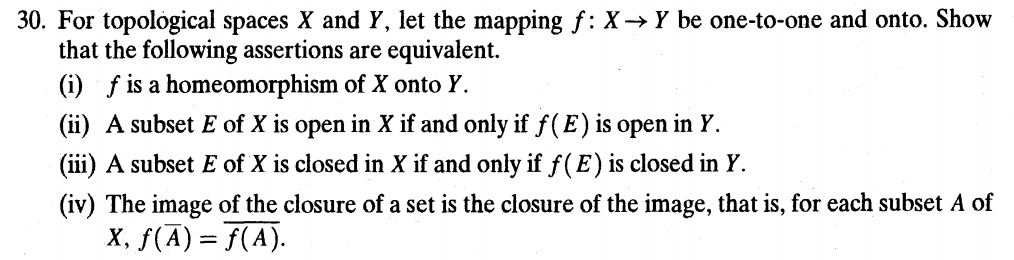
\includegraphics[width=1\textwidth]{11-30}
\end{figure}
\end{question}
\begin{solution}
Assume (i). We claim that $f(\bar{A}) \subseteq \overline{f(A)}$. Let
$y \in f(\bar{A})$. Then, there exists $x \in \bar{A}$, such that
$f(x) = y$. Since $f$ is homeomorphic, it is continuous. 
By continuity of $f$ at $x$, for any neighborhood $O$
of $y$, there exists a neighborhood $U$ of $x$, such that $f(U) \subseteq 
O$. As $x \in \bar{A}$, $U \cap A \neq \emptyset$, and $f(U) \cap f(A) 
\neq \emptyset$. Since $f(U) \subseteq O$, $f(A) \cap O \neq \emptyset$. 
Hence, $y \in \overline{f(A)}$. We now claim that
$\overline{f(A)} \subseteq f(\bar{A})$. Let $y \in \overline{f(A)}$.  


\smallskip

Assume $(ii)$, and let $E$ be a closed subset of $X$. We have $X \setminus E$
is open. By $(ii)$, $f(X\setminus E)$ is open. As $f$ is surjective, 
we have $f(X) = Y$. It follows that
\eQb
f(X\setminus E) &=& f(X) \setminus f(E) \\
&=& Y \setminus f(E). 
\eQe
Since $Y \setminus f(E)$ is open, $f(E)$ is closed. 

\smallskip

\end{solution}

\newpage

\begin{question}[2. Royden 11-34]
\hfill
\begin{figure}[h!]
  \centering
    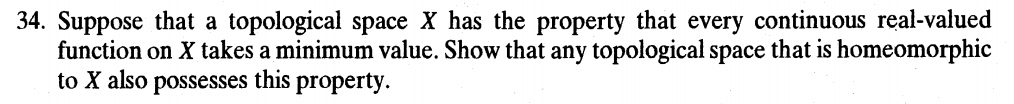
\includegraphics[width=1\textwidth]{11-34}
\end{figure}
\end{question}
\begin{solution}
Let $Y$ be a topological space that is homeomorphic to $X$, and
$\phi:X \to Y$ be a bijective map such that $\phi^{-1}$ is continuous.
Let $g$ be a continuous real-valued function, defined on $Y$. Consider
$g(Y)$. We wish to show that $\inf_{y \in Y} g(y) \in g(Y)$.  

\end{solution}

\newpage

\begin{question}[3. Royden 11-44]
\hfill
\begin{figure}[h!]
  \centering
    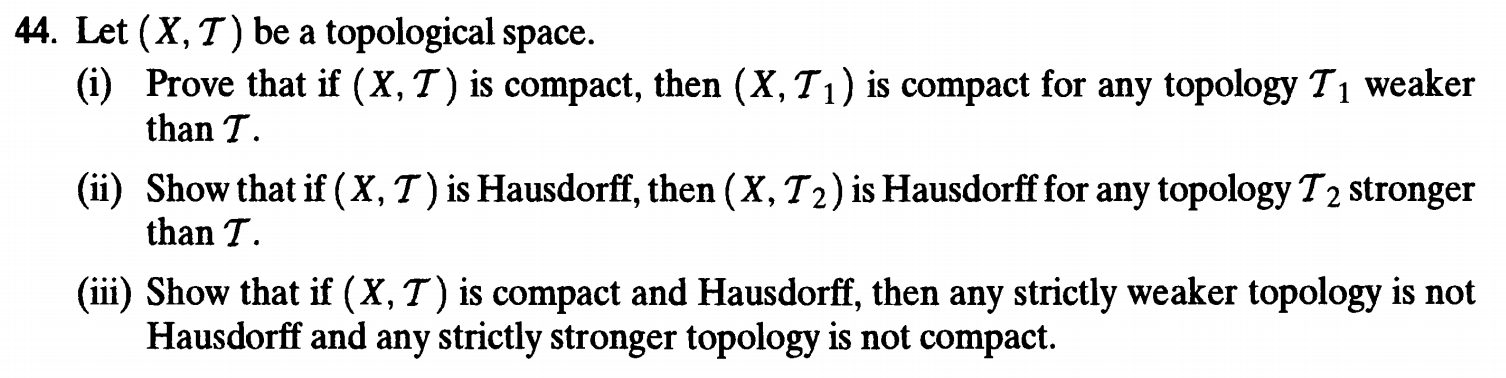
\includegraphics[width=1\textwidth]{11-44}
\end{figure}
\end{question}
\begin{solution} 
\textbf{(i)} 
Let $\mathscr{T}_1$ be a topology for $X$, that is weaker than $\mathscr{T}$.
It follows that $\mathscr{T}_1 \subseteq \mathscr{T}$. Let $E$ be
a subset of $X$, and $\{O_\lambda \}_{\lambda \in \Lambda}$ be 
an open cover of $E$ in $(X,\mathscr{T}_1)$. 
As $\mathscr{T}_1 \subseteq \mathscr{T}$, 
the considered open cover is also an open cover in $(X,\mathscr{T})$. 
By compactness of $(X,\mathscr{T})$, 
there exists a finite sub-collection of the open cover, that covers $E$.
Hence, $(X,\mathscr{T}_1)$ is compact. \hfill $\qed$ 

\smallskip

\textbf{(ii)}
Let $\mathscr{T}_2$ be a topology for $X$, that is stronger than 
$\mathscr{T}$. It follows that $\mathscr{T} \subseteq \mathscr{T}_2$. 
If $|X| < 2$, $X$ with any topology is trivially Hausdorff. Hence,
we only consider the remaining case of $|X| \geq 2$. 
Let $x,y \in X$ such that $x \neq y$. As $(X,\mathscr{T})$ is Hausdorff,
there exists a neighborhood of $x$, and a neighborhood of $y$, that are
disjoint, which we denote as $U$ and $V$ respectively. As 
$\mathscr{T} \subseteq \mathscr{T}_2$, $U$ and $V$ are also open in 
$(X,\mathscr{T}_2)$. Hence, $U$ is a neighborhood of $x$, and $V$
is a neighborhood of $y$ in $(X,\mathscr{T}_2)$. Moreover, $U$ and $V$ are
disjoint. Hence, $(X,\mathscr{T}_2)$ is Hausdorff. \hfill $\qed$
 
\smallskip

\textbf{(iii)} 
Let $\mathscr{T}_1$
be a topology for $X$, that is strictly weaker than $\mathscr{T}$. It follows
that there exists a subset $E$ of $X$ such that it is open in 
$(X,\mathscr{T})$, but not open in $(X,\mathscr{T}_1)$. Furthermore, 
$X \setminus E$ is closed in $(X,\mathscr{T})$, but not closed in
$(X\mathscr{T}_1)$. As $(X,\mathscr{T})$ is compact, $X \setminus E$
is compact as a subspace.
Since $\mathscr{T}_1$ is weaker than $\mathscr{T}$, 
$X\setminus E$ is compact. 
Suppose for sake of contradiction that $(X,\mathscr{T}_1)$
is Hausdorff. It implies that $X \setminus E$ is closed in
$(X,\mathscr{T})$, which is a contradiction. Hence, $(X,\mathscr{T}_1)$
is not Hausdorff. \hfill $\qed$

\smallskip
 
Let $\mathscr{T}_2$ be a topology for $X$, that is strictly stronger than
$\mathscr{T}$. It follows that there exists a subset $E$ of $X$ such that
it is open in $(X,\mathscr{T}_2)$, but not open in $(X,\mathscr{T})$. 
Furthermore, $X\setminus E$ is closed in $(X,\mathscr{T}_2)$, but not
closed in $(X,\mathscr{T})$. Suppose for sake of contradiction that 
$(X,\mathscr{T}_2)$ is compact. Then, as $X \setminus E$ is closed in $(X,
\mathscr{T}_2)$ is compact. As $\mathscr{T}$ is weaker than 
$\mathscr{T}_2$, $X \setminus E$ is compact in $(X,\mathscr{T})$. As
$(X\mathscr{T})$ is Hausdorff, $X\setminus E$ is closed in $(X,\mathscr{T})$,
which is a contradiction. Hence, $(X,\mathscr{T}_2)$ is not compact. 
\hfill $\qed$ 
\end{solution}

\newpage

\begin{question}[4. Royden 11-46]
\hfill
\begin{figure}[h!]
  \centering
    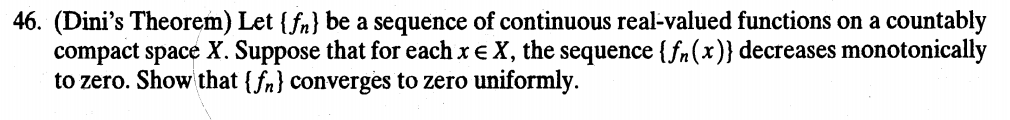
\includegraphics[width=1\textwidth]{11-46}
\end{figure}
\end{question}
\begin{solution}

\end{solution}

\pagebreak

\begin{question}[4. Royden 12-16]
\hfill
\begin{figure}[h!]
  \centering
    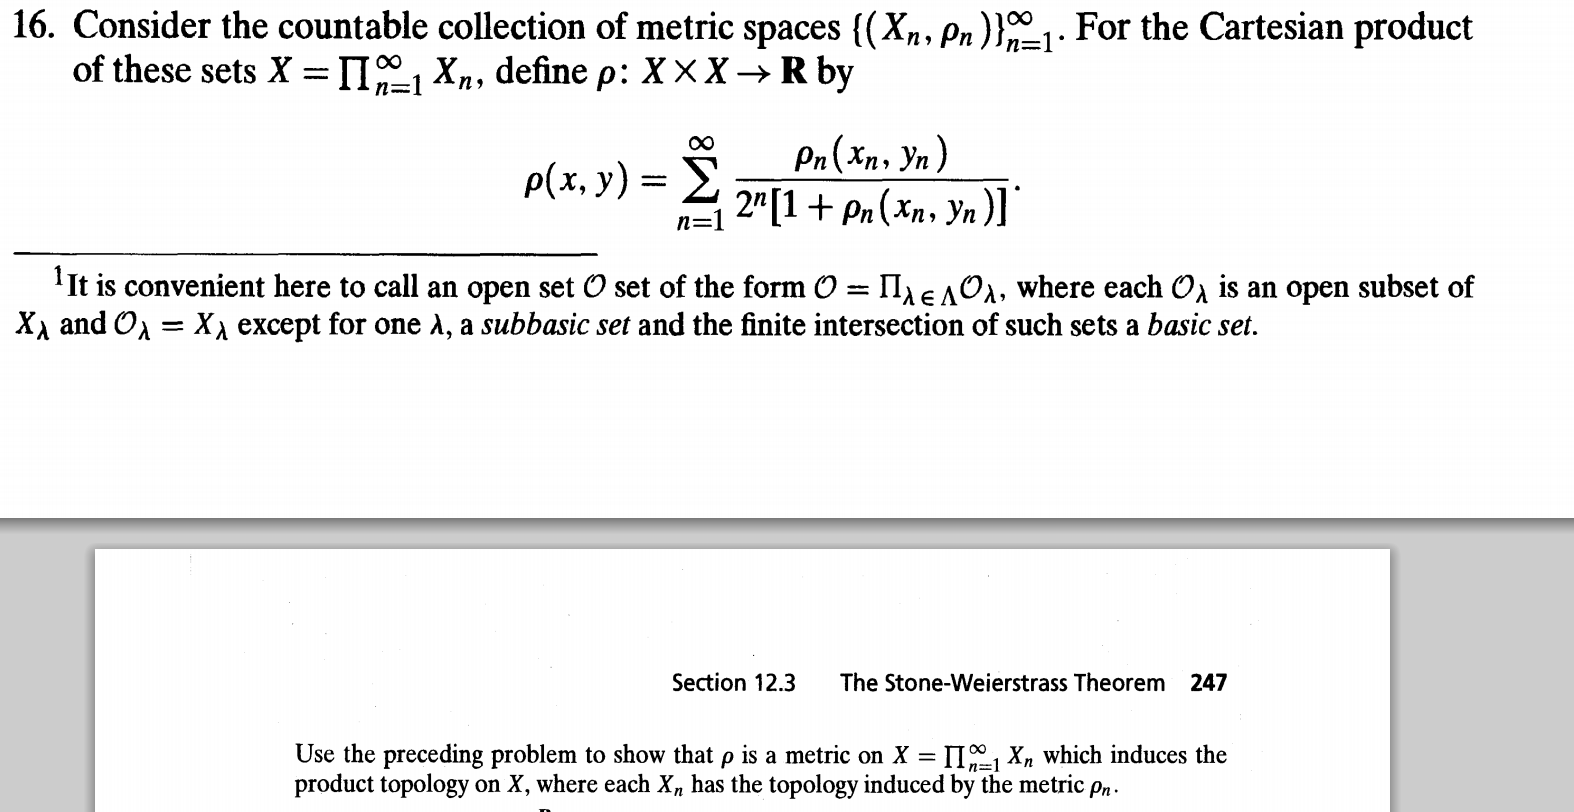
\includegraphics[width=1\textwidth]{12-16}
\end{figure}
\end{question}
\begin{solution}
\end{solution}

\pagebreak

\begin{question}[6. Royden 12-20]
\hfill
\begin{figure}[h!]
  \centering
    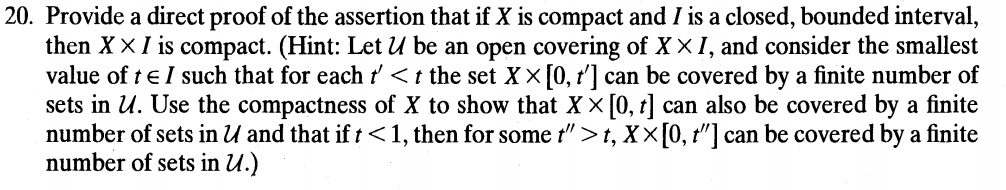
\includegraphics[width=1\textwidth]{12-20}
\end{figure}
\end{question}
\begin{solution}
\end{solution}


\end{document}
